\documentclass[a4paper,10pt]{paper}

\usepackage[utf8]{inputenc}
\usepackage{graphicx}
\usepackage{amsmath}
\usepackage{amsfonts}

\begin{document}

\title{Satogaeri}
\author{Markus Leitner}
\maketitle 
\tableofcontents

\section{Introduction}



\section{Satogaeri}
Satogaeri is a logic puzzle published by the Japanese company Nikoli Co.m Ltd. in 2002. Satogaeri only made a booklet appearance in Nikoli Vol. 99, Vol. 100 and Vol. 101. However it got revived on nikoli.com in 2013.

\subsection{Rules}
The official rules from Nikoi state:

\begin{enumerate}
  \item The areas enclosed by bold lines, are called "Countries." Move the circles, vertically or horizontally, so each country contains only one circle.
  \item The numbers in the circles indicate how many cells they have to pass through. Circles without numbers may move any distance, but some of them do not move.
  \item The circles cannot cross the tracks of other circles and cannot go over other circles. 
\end{enumerate}
And additionally the 4th rule, which counts for every logic puzzle:
\begin{enumerate}
  \item[4] A puzzle only has one solution.
\end{enumerate}

\begin{figure}
  \centering
  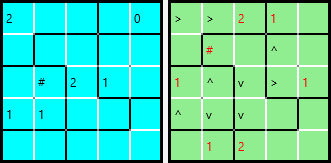
\includegraphics[width=0.9\textwidth]{Pictures/sample_small.png} 
  \caption{Small sample puzzle with its solution}
  \label{fig:sample_small}
\end{figure}

Handcrafted puzzles tend to have a mirrored country-layout either vertically, horizontally or both as can be seen in Figure~\ref{fig:sample_small}. Numberless Circles are here referred to as '\#'.

\section{Satisfiability Modulo Theories}
Before we can go on and talk about how to solve Satogaeri problems we first have to look intt Satisfiability Modulo Theories (SMT) for this was used to create the solver and the generator.

SMT can be seen as an enhancement of the traditional Satisfiability (SAT) solving. In SAT solving one tries to find an interpretation of a given problem, where this interpretation is a boolean formula composed of boolean variables and expressions like AND, OR and NOT; to state a few. If this constructed formula has a configuration of its variables where the formula evaluates to 'true', then also the original problem must have a solution. A satisfying configuration of the variables often gives a good clue on how to solve the original problem.
To state an example: the formula
\[(a \lor b \lor (\neg c)) \iff ((\neg a) \land c)\]
is satisfied with the assignment \textit{a} is 'false', \textit{b} and \textit{c} are 'true'. Therefore the originating problem of this formula must be solvable too.
SMT goes one step beyond that by replacing some boolean variables with predicates. A predicate is basically a binary-valued function of non-binary variables, which allows us to have function symbols with different arities. Now we can express formulas in first-order logic like
\[x > y \land 3 x + 4 \leq 4 y\]
where a natural number can be seen as a function symbol with arity 0, a so called constant.
There are many different approaches of implementing SMT solvers, but the two major ones are the \textit{eager} and the \textit{lazy} approach.
\subsection{Eager SMT}
In the \textit{eager} approach one tries to convert the given formula into an equisatisfiable propositional formula with all the additional needed constraints of the originating problem. With this constraints the search-space should be reduced so that a common SAT solver can solve the formula much quicker. And this is the appealing part of thes approach: one can use already existing SAT solver to finally check the satisfiability. However the converting process into a propositional formula can be cost-intensive.\cite{2009satisfiability}
\subsection{Lazy SMT}
The \textit{lazy} approach consists of two parts. The first part are theory-specific solvers ($\mathcal{T}$-solvers) to handle conjunctions of literals, which are embedded again into a SAT solver. The advantage of incorporating $\mathcal{T}$-solvers is that one can use a specific algorithm and data-structure which fits the problem at hand best. This should lead to a better performance.\cite{sebastiani2007lazy}

\subsection{SMT-Library}
The SMT-Library (SMT-Lib) was found in 2003 to provide common standards and a library of benchmarks for diverse SMT-Solvers. With this standards and benchmarks evaluation and comparison of SMT-Systems should be made easier to give the research a competitive touch, which ultimately should result in advancing the state of the art in the SMT-Field. They even organize an annually SMT-Solver competition (SMT-COMP).
SMT-Lib was greatly useful for this thesis by providing an easily understandable syntax which made many SMT-Solver accessible, like Boolector, CVC4 and MathSAT 5 to state a few. On their web-site\footnote{www.SMT-LIB.org} one can find a long list of Solver supporting SMT-LIB and a separate list of these Solver still under active development.

\subsection{Logics}
SMT-LIB supports a huge variety of different logics. The advantage here is to be able to apply more specialized and therefore more efficient algorithms.
\begin{figure}
  \centering
  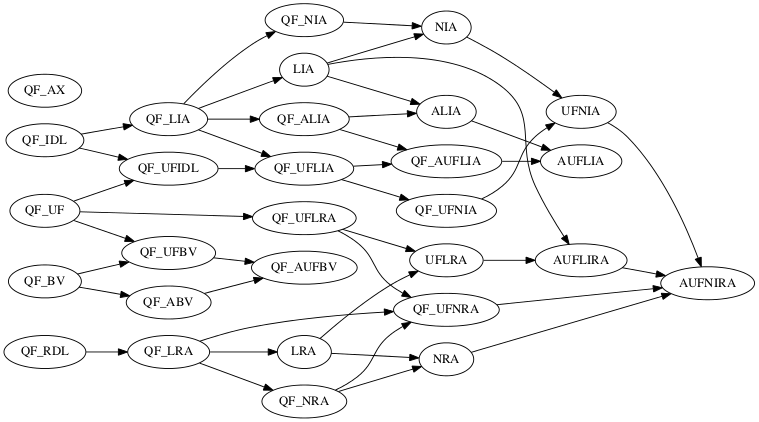
\includegraphics[width=0.9\textwidth]{Pictures/logics.png}  
  \caption{A link from a logic L1 to a logic L2 means that every formula of L1 is also a formula of L2}
  \label{fig:logics}
\end{figure}
The meaning of the logics in Figure~\ref{fig:logics} is letter coded. For example:
\begin{enumerate}
  \item QF stands for the restriction to quantifier free formulas
  \item IA stands for the theory Ints (Integer Arithmetic)
  \item L before IA, RA, or IRA stands for the linear fragment of those arithmetics 
\end{enumerate}
So QF\_LIA is an unquantified linear integer arithmetic. In essence, Boolean combinations of inequations between linear polynomials over integer variables.
The whole explanation can be found on the SMT-Lib web-site\footnote{www.SMT-LIB.org} in the section Logics.

\subsection{CVC4}
The SMT-Solver used in this project is the Cooperating Validity Checker 4 (CVC4), currently the most novel  successor of the Stanford Validity Checker which was found in 1996. CVC4 is a joined project of the New York University and the University of Iowa.
Supported features are inter alia: several built-in base theories, support of quantifiers and a model generation ability. The latter is a very important requirement for this project at hand.
Furthermore CVC4 has its own wiki-web-page\footnote{http://cvc4.cs.nyu.edu/wiki} with useful tutorials, user manual and an developer section.


\section{The Solver}



\section{The Generator}

\subsection{Drawing}

\section{Statistics}

\section{JavaFX}

\section{Conclusion}


\end{document}
% eager SMT
@article{barrett2009satisfiability,
  title={Satisfiability Modulo Theories.},
  author={Barrett, Clark W and Sebastiani, Roberto and Seshia, Sanjit A and Tinelli, Cesare},
  journal={Handbook of satisfiability},
  volume={185},
  pages={825--885},
  year={2009}
}
% lazy SMT
@article{sebastiani2007lazy,
  title={Lazy satisfiability modulo theories},
  author={Sebastiani, Roberto},
  year={2007},
  publisher={University of Trento}
}